\section{Problem 2-2 Three-Dimensional Lattice Net\-work}

Consider an undirected network $G = (V,E)$ with $N = \ell^3$ nodes corresponding to points on a regular three-dimensional lattice $\{1,...,\ell\}\times\{1,...,\ell\}\times\{1,...,\ell\}$. Two nodes $x$ and $y$ are connected if and only if $d(x,y) = 1$, where $d(x,y)$ denotes the Euclidean distance. A visualization of such a graph is shown in the following image:

\begin{figure}[ht]
	\centering
	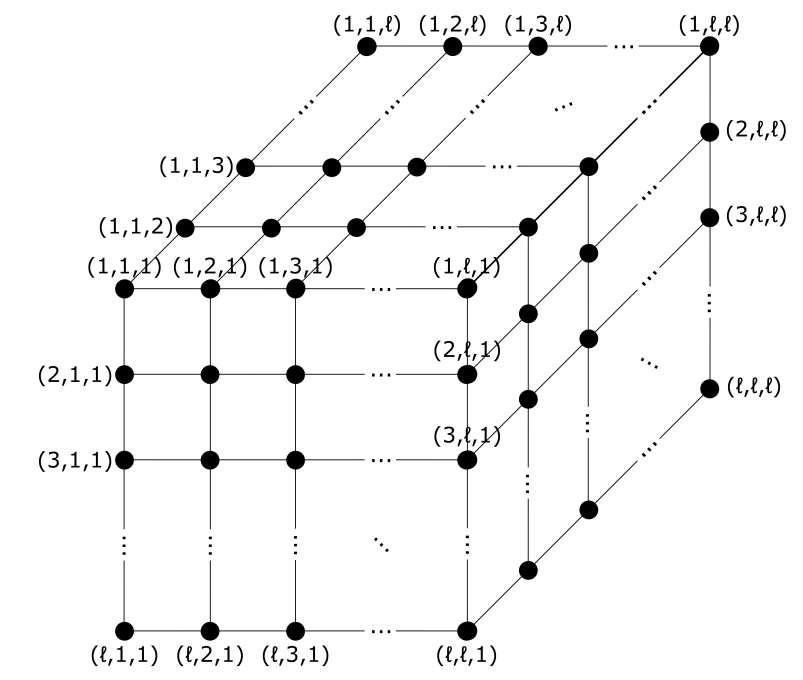
\includegraphics[width=0.7\linewidth]{images/lattice.png}
	\caption{Three-Dimensional Lattice Network}
	\label{fig:lattice}
\end{figure}

\begin{enumerate}
	\item What is the diameter $d_{max}$ of the graph?
	\vspace{0.25cm}
	
	The diameter is the longest shortest path in the graph. One example for a longest shortest path is the distance from the left upper edge in the front $(1,1,1)$ to the right lower edge in the back $(\ell,\ell,\ell)$. The diameter is therefore $d_{max} = 3\ell$.
	
	\item Provide an expression (in terms of $N$ and/or $\ell$) for the probability $p_i$ that a randomly chosen node has degree $i$. You may assume that $\ell \geq 3$. What are the consequences for $N \rightarrow \infty$?
	\vspace{0.25cm}
	
	Due to the fact that there are four different types of nodes (inner nodes, corner nodes, edge nodes and outer nodes) with differing degree three different expressions are provided in the following.
	
	\newpage
	
	First the distribution of the different node types is clarified in table \ref{tab:node_distribution}:
	
	\begin{table}[h]
	\centering
	\begin{tabular}{l|l|l}
		\hline
		\rowcolor{lightgray}
		Node type & edges & nodes \\ 
		\hline
		inner node    & 6 & $(\ell-2)^3$ \\
		\hline
		corner node    & 3 & $8$ \\
		\hline
		edge node    & 4  & $12 \ell - 8$ \\
		\hline
		outer node    & 5  & $6*\ell^2 - 12*\ell$ \\
		& & (nodes on all six sides: $6*\ell^2$ \\
		& & substract all edge nodes: $-12*\ell$) \\
		\hline
	\end{tabular}
	\caption{}
	\label{tab:node_distribution}
	\end{table}

	Secondly the expressions for the probability distribution are derived based on the following formula with $N=\ell^3$ and $p=\frac{\#nodes}{\ell^3}$:
	
	\begin{equation}
	p_k = {{N-1}\choose{k}} * p^k * (1-p)^{N-1-k}
	\end{equation}
	
	For inner nodes with $i=6$:
	\begin{equation}
	p_6 = {{\ell^3-1}\choose{6}} * (\frac{(\ell-2)^2}{\ell^3})^6 * (1-{\frac{(\ell-2)^2}{\ell^3}})^{\ell^3-1-6}
	\end{equation}
	
	For corner nodes with $i=3$:
	\begin{equation}
	p_3 = {{\ell^3-1}\choose{3}} * ({\frac{8}{\ell^3}})^3 * (1-{\frac{8}{\ell^3}})^{\ell^3-1-3}
	\end{equation}
	
	For edge nodes with $i=4$:
	\begin{equation}
	p_4 = {{\ell^3-1}\choose{4}} * ({\frac{12 \ell - 8}{\ell^3}})^4 * (1-{\frac{12 \ell - 8}{\ell^3}})^{\ell^3-1-4}
	\end{equation}
	
	For outer nodes with $i=5$:
	\begin{equation}
	p_4 = {{\ell^3-1}\choose{5}} * ({\frac{6*\ell^2 - 12*\ell}{\ell^3}})^5 * (1-{\frac{6*\ell^2 - 12*\ell}{\ell^3}})^{\ell^3-1-5}
	\end{equation}
	
	For $N \rightarrow \infty$ also $\ell \rightarrow \infty$, that is why the probability for an inner node increases and the probability for a corner or a border node decreases.
	
	\item What is (i) the clustering coefficient of a node i and (ii) the average clustering coefficient of this network?
	\vspace{0.25cm}
	
	(i) the clustering coefficient of a node i
	
	The clustering coefficient is defined as:
	\begin{equation}
	C_i = \frac{2*L_i}{k_i * (k_i-1)}
	\end{equation}
	with $L_i$ being the number of edges between the neighbors of the node and $k_i$ being the degree from the chosen node.
	
	The clustering coefficient is 0 for all types of nodes, because there are no edges (diagonal edges between the nodes) between the neighbors of the node ($L_i = 0$).
	
	(ii) the average clustering coefficient of this network
	
	The average clustering coefficient is defined as:
	\begin{equation}
	\langle C \rangle = \frac{1}{N} \sum_{i=1}^{N} C_i
	\end{equation}
	
	As described in (i) the clustering coefficient is zero for all nodes. Con\-se\-quent\-ly the average clustering coefficient is also zero.
	
	\item Now assume we have a different three-dimensional lattice graph with nodes corresponding to points $\{1,...,\ell\}\times\{1,...,\ell\}\times\{1,...,\ell\}$, where two nodes $x$ and $y$ are connected if and only if $d(x,y) \leq \sqrt{3}$. How	does this change the average clustering coefficient in the limit $N \rightarrow \infty$?
	\vspace{0.25cm}
	
	Now diagonal edges between the nodes are present. That is why the clustering coefficient is not zero any more.
	
	For $N \rightarrow \infty$: it is sufficient to only look at the inner nodes: 
	
	\begin{equation}
	L_i = \frac{16*6 (inner) + 10*12 (edge) + 6*8 (corner)}{2}
	\end{equation}
	
	\begin{equation}
	k_i = 3*3*3-1 = 26
	\end{equation}
	
	\begin{equation}
	C_i = \frac{2*L_i}{k_i * (k_i-1)}
	\end{equation}
	
	\begin{equation}
	\langle C \rangle \rightarrow 0,24
	\end{equation}
	
\end{enumerate}